\documentclass[9pt,aspectratio=169]{beamer}
\mode<presentation>
\usepackage[T1]{fontenc}
\usepackage{color}
\usepackage{graphicx}
\usepackage{natbib}
\usepackage{tikz}
\usetikzlibrary{shapes.geometric}
\usepackage{xmpmulti}
\usepackage{animate}
\usepackage{tcolorbox}
\usepackage{amsmath}
\usepackage{xcolor, soul}
\usepackage{gensymb}
\usepackage{appendixnumberbeamer}

%\definecolor{links}{HTML}{2A1B81}
%\hypersetup{urlcolor=links} % Does not apply color to href's
%\hypersetup{colorlinks,urlcolor=links} 

\usetheme{Boadilla}
%\usecolortheme{seahorse}

\usefonttheme{professionalfonts}

\title[Stopping Criteria]{Statistical stopping criteria for automated screening in systematic reviews}
\date{20 October 2022}
\author{Finn Müller-Hansen, Max Callaghan}
\institute[MCC]{
	
\includegraphics[height=1cm,width=2cm]{images/MCC_Logo_RZ_rgb.jpg}
}



\newtheorem*{remark}{}


\bibliographystyle{apalike}

\begin{document}
	\begin{frame}
	\titlepage
\end{frame}

%%%%%%%%%%%%%%%%%%%%%%
% Motivation
%\begin{frame}{Motivation}
%
%\end{frame}

%%%%%%%%%%%%%%%%%%%%%%
% RITL
\begin{frame}{Researcher in the Loop process}

\begin{columns}
	\begin{column}{0.618\linewidth}
		\begin{itemize}
			\item<1-> A large literature \citep{omara-eves_using_2015} has developed ``human-in the loop'' machine learning applications which ``overcome the manual and time-consuming screening of large numbers of studies by prioritizing relevant studies via active learning''  \cite{van_de_schoot_open_2021}
			\item<2-> Identifying 95\% of relevant documents if screening manually would mean screening 95\% of all documents
			\item<3-> If we can use machine learning to prioritise documents likely to be relevant, we can achieve high levels of recall with low levels of effort.
			\item<4-> BUT, given we do not know \textit{a priori} the true number of relevant documents, we need strategies to stop screening and bank the work savings
			\item<5->Getting these wrong can mean missing our target
		\end{itemize}
	\end{column}
	\begin{column}{0.382\linewidth}
		\begin{figure}
			\only<2-3>{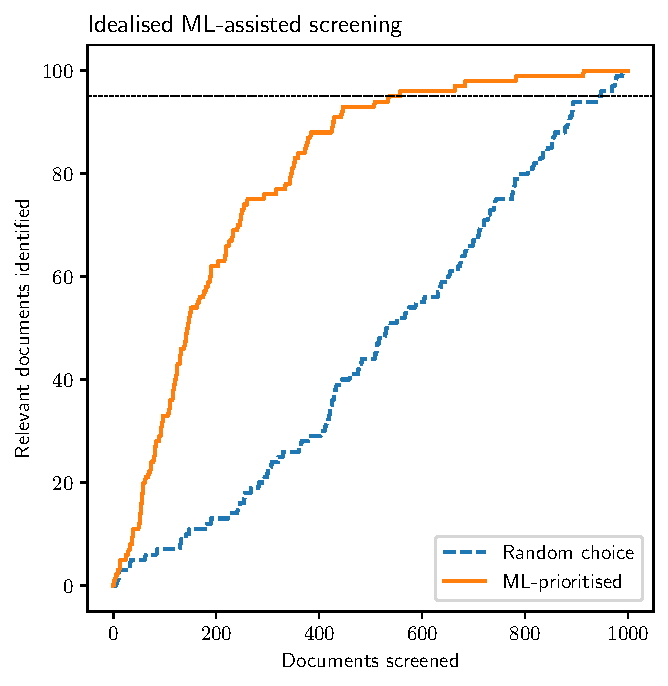
\includegraphics[width=\linewidth]{images/idealised_stopping.pdf}}
			\only<4>{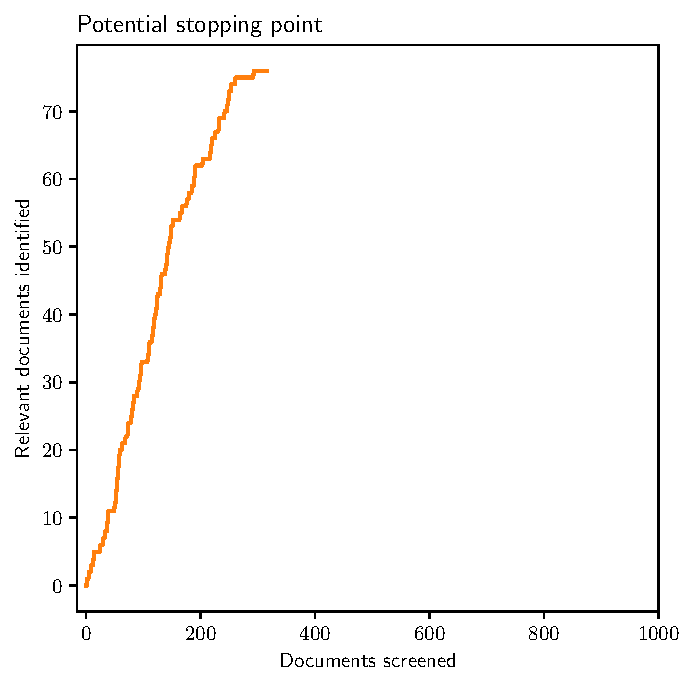
\includegraphics[width=\linewidth]{images/potential_stopping.pdf}}
			\only<5>{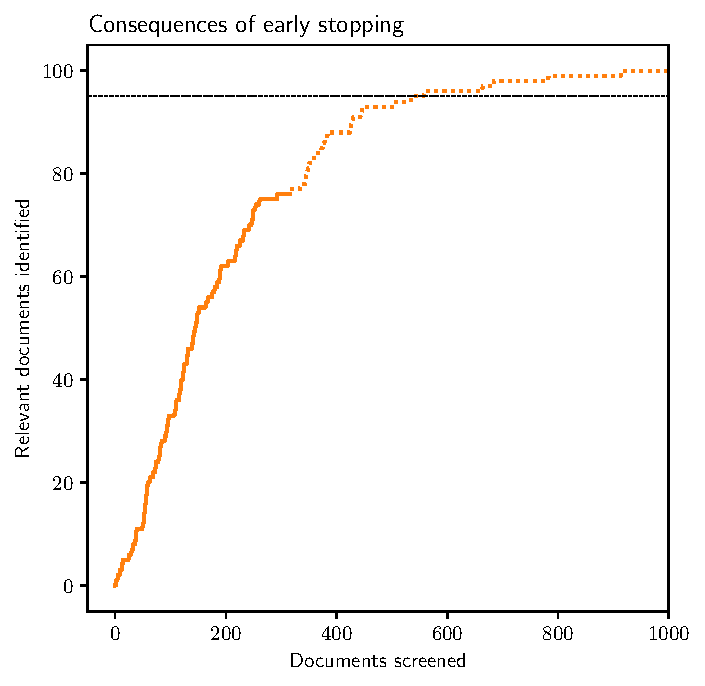
\includegraphics[width=\linewidth]{images/early_stopping.pdf}}
%			\only<2>{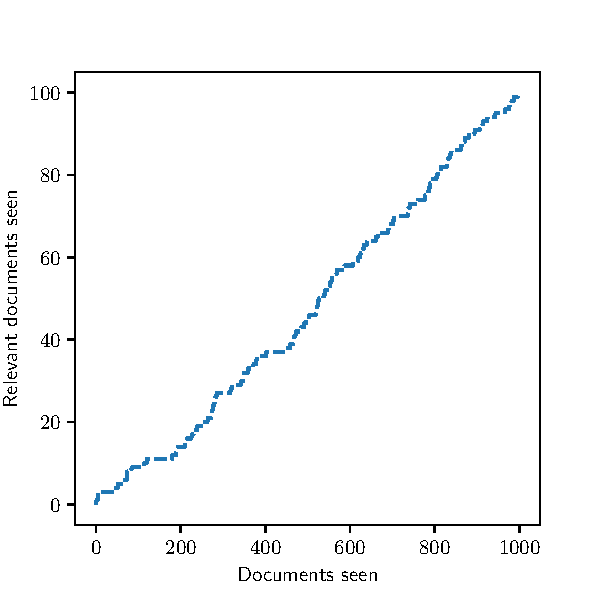
\includegraphics[width=\linewidth]{images/random.pdf}}
%			\only<3>{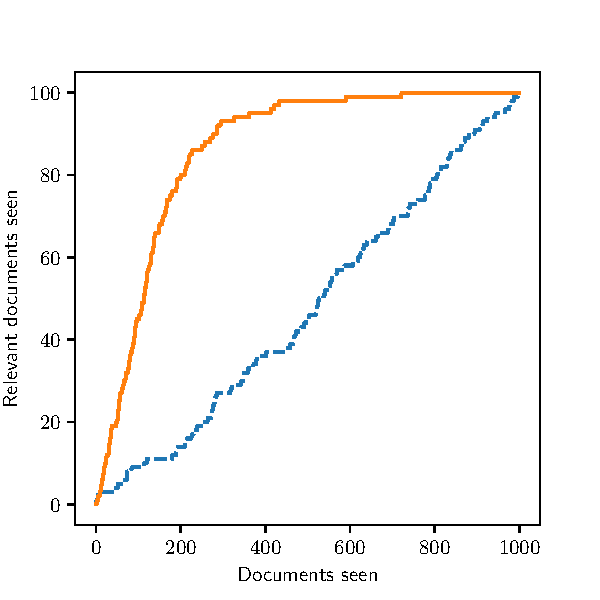
\includegraphics[width=\linewidth]{images/ml_prio.pdf}}
%			\only<4>{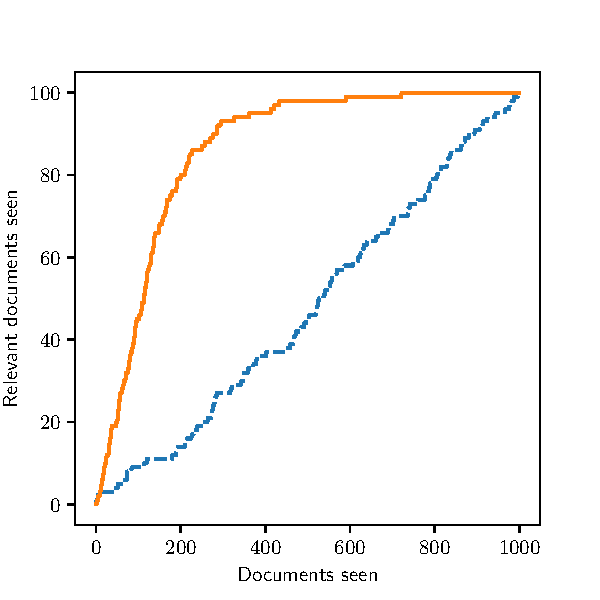
\includegraphics[width=\linewidth]{images/ml_prio.pdf}}
		\end{figure}
	\end{column}
\end{columns}

\end{frame}

%%%%%%%%%%%%%%%%%%%%%%
% Urn
\begin{frame}{A stopping criterion}



\begin{columns}
	
	\begin{column}{0.382\linewidth}
		\begin{figure}
			\only<1-3>{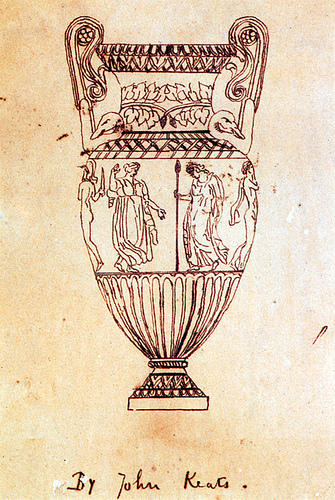
\includegraphics[width=.8\linewidth]{images/Keats_urn.jpg}}
			\only<4->{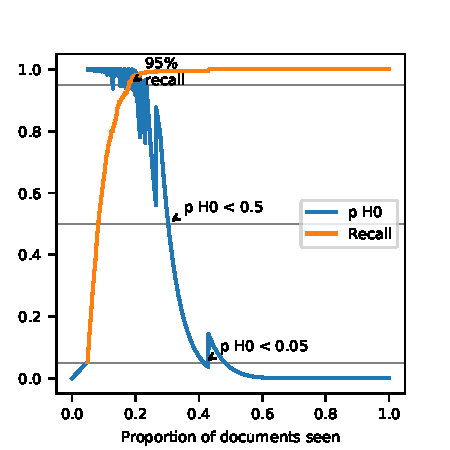
\includegraphics[width=\linewidth]{../images/h0_paths_ProtonBeam.pdf}}
			
		\end{figure}
	\end{column}
	\begin{column}{0.618\linewidth}
		\begin{itemize}
			\item<1-> Our stopping criterin works by treating documents as if they were white (not relevant) and red (relevant) marbles drawn from an urn without replacement.
			\item<2-> The hypergeometric distribution tells us the probability of observing \textbf{k} red marbles in a sample of \textbf{n} marbles, given an urn with \textbf{N} marbles, of which \textbf{K} are relevant
			\item<3-> We reformulate this to generate a null hypothesis $H_0$ that a given recall target has been \textbf{missed}. 
			\item<4-> We calculate a p-score for our null hypothesis, and if this is low enough, we reject $H_0$ and stop screening.
		\end{itemize}
	\end{column}

\end{columns}

\medskip

\bigskip

\only<5->{Note, ML-prioritisation means documents are not drawn at random, which makes our test conservative as long as ML works as well as or better than random chance.}

\end{frame}


%%%%%%%%%%%%%%%%%%%%%%
% Results
\begin{frame}{Results}

We test our criteria against other commonly used criteria on 20 complete systematic review datasets

\begin{columns}
	\begin{column}{0.618\linewidth}
		\begin{itemize}
			\item<1-> \textit{Potential} work savings (if we already knew when to stop) varied widely (higher for larger datasets - blue dots)
			\item<2-> Existing stopping criteria can result in catastrophic errors
			\item<4-> Our criteria generated work savings with reliably conservative performance wrt our recall target.
		\end{itemize}
	\end{column}
	\begin{column}{0.382\linewidth}
		\begin{figure}
			\only<1>{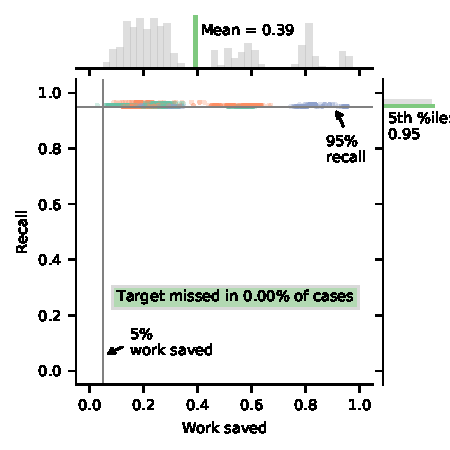
\includegraphics[width=\linewidth]{../manuscript/2_figs_jointplot_pf.pdf}
				\caption{A priori knowledge}
			}
			\only<2>{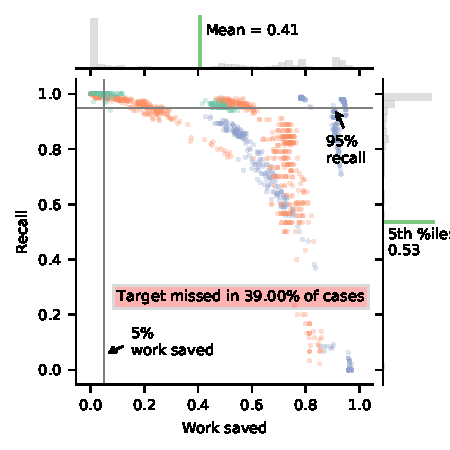
\includegraphics[width=\linewidth]{../manuscript/2_figs_jointplot_ih_50.pdf}
				\caption{50 consecutive irrelevant articles}
			}
			\only<3>{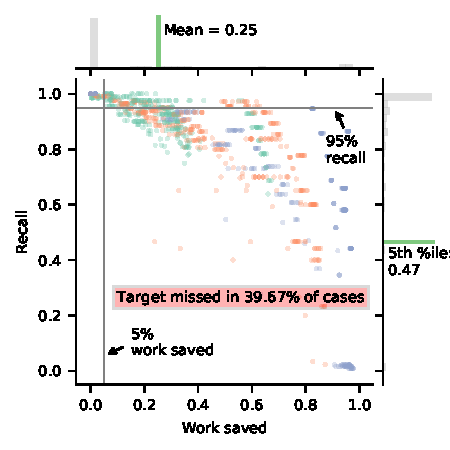
\includegraphics[width=\linewidth]{../manuscript/2_figs_jointplot_bir.pdf}
				\caption{Estimating baseline inclusion rate}
			}
			\only<4>{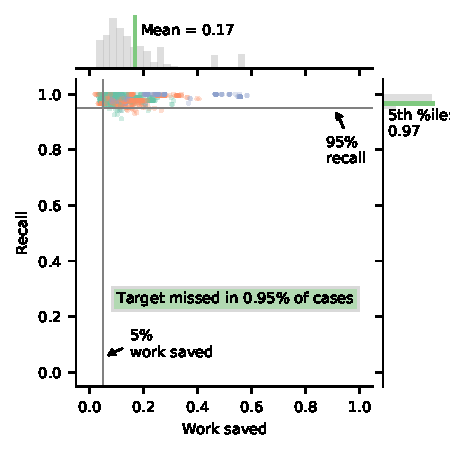
\includegraphics[width=\linewidth]{../manuscript/2_figs_jointplot_nrs.pdf}
				\caption{Our criterion}
			}

		\end{figure}
	\end{column}
\end{columns}


\end{frame}


%%%%%%%%%%%%%%%%%%%%%%
% Conclusion
\begin{frame}{Conclusion}

We provide a stopping criteria that works on any model, with any tool: \url{https://github.com/mcallaghan/rapid-screening/blob/master/analysis/hyper_criteriaR.md}.

\medskip

Work savings in practice with large datasets are large!

\medskip

Future work will identify how biased our urn is, in order to use a noncentral hypergeometric distribution, which should give a more precise, less conservative criterion.

\begin{center}
	\line(1,0){250}
	
	\medskip
	
	\textbf{Thanks!}
	
	\medskip
	
	Contact: \url{mueller-hansen@mcc-berlin.net, callaghan@mcc-berlin.net}
	
	Twitter: \url{https://twitter.com/MaxCallaghan5}
	
\end{center}

\end{frame}

%%%%%%%%%%%%%%%%%%

\appendix


\begin{frame}{References}

\bibliography{rapid-review}

\end{frame}

\begin{frame}{Applications and extensions}

\begin{columns}

\column{0.33\textwidth}
\only<1->{
	\begin{figure}
		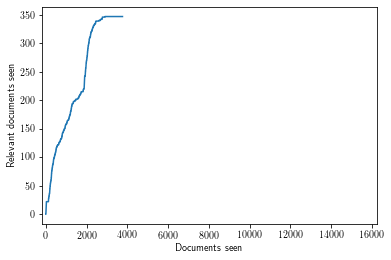
\includegraphics[width=\linewidth]{images/doebbeling_ws.png}
	\end{figure}
}

\column{0.33\textwidth}
\only<2->{
	\begin{figure}
		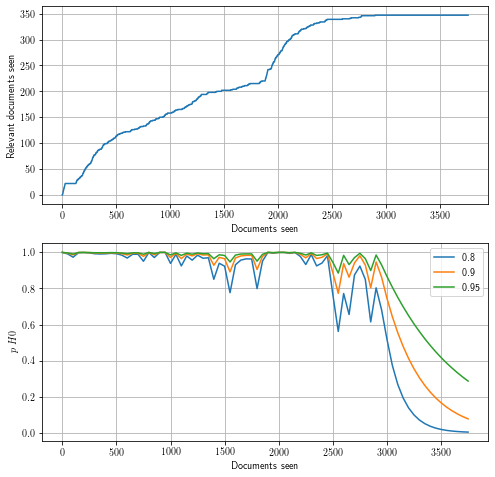
\includegraphics[width=\linewidth]{images/doebbeling_p.png}
	\end{figure}
}


\column{0.33\textwidth}

\small

\begin{itemize}
	\item<1-> We have used the stopping criteria to generate massive savings (77\%) in real projects
	\item<2-> If rejecting our $H_0$ was less labour intensive we could have saved around 82\%
	\item<3-> Using a biased urn could help create a more precise criterion
\end{itemize}

\end{columns}

\end{frame}			

%%%%%%%%%%%%%%%%%%%%%%
% Other criteria
\begin{frame}{Baseline Inclusion Rate}

\begin{columns}
	\begin{column}{0.618\linewidth}
		\begin{itemize}
			\item<1-> If we try to estimate the baseline inclusion rate, we will get it wrong most of the time. Overestimating results in 0 work savings, while underestimating results in less than target recall.
			\item<2-> Wrongness decreases with larger sample sizes, but bad outcomes remain most frequent.
		\end{itemize}
	\end{column}
	\begin{column}{0.382\linewidth}
		\begin{figure}
			\only<1>{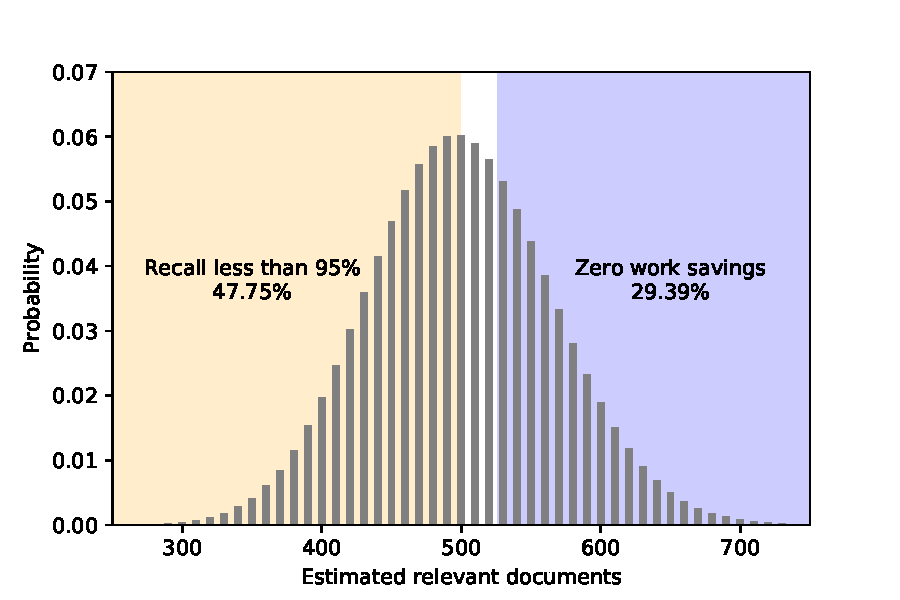
\includegraphics[width=\linewidth]{../manuscript/2_figs_bir_errors.pdf}
			}
			\only<2>{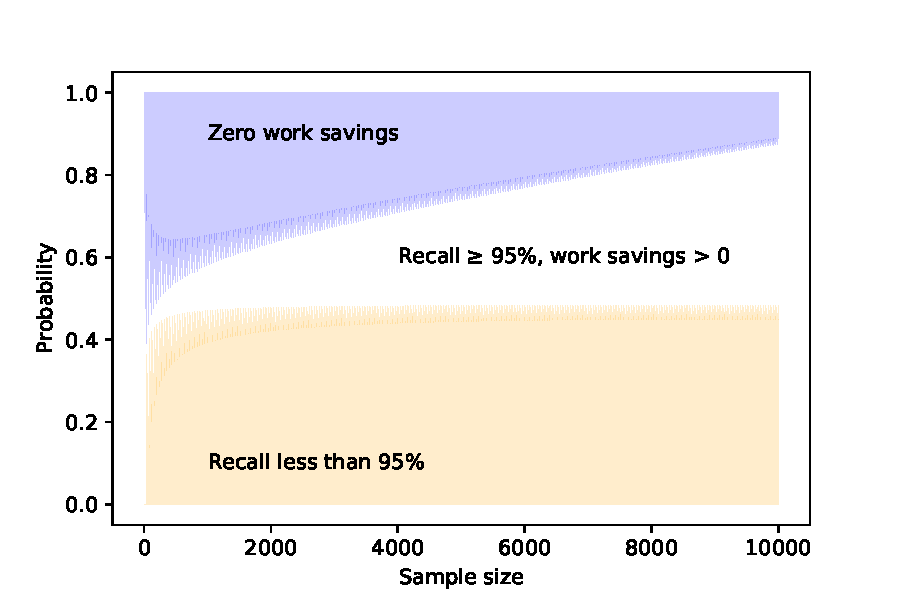
\includegraphics[width=\linewidth]{../manuscript/2_figs_bir_error_distribution.pdf}
}
			
		\end{figure}
	\end{column}
\end{columns}

\end{frame}

\begin{frame}{Theory I}
We form a null hypothesis that the target level of recall has not been achieved

\begin{equation}
H_0 : \tau < \tau_{tar}
\end{equation}

To operationalise this, we come up with a hypothetical value of $K$ which is the lowest value compatible with our null hypothesis

\begin{equation}
K_{tar} = \lfloor \frac{\rho_{seen}}{\tau_{tar}}-\rho_{AL}+1 \rfloor
\end{equation}

In other words, if there were $K_{tar}$ or more relevant documents in the urn when sampling began, the $\rho_{al}$ relevant we identified before sampling, and the $k$ we drew from the urn would not be enough to meet our target recall level.

\medskip 

The cumulative distribution function gives us the probability of observing what we observed, if our null hypothesis were true

\begin{equation}
p = P(X \leq k) \text{, where } X \sim Hypergeometric(N,K_{tar},n)
\label{eq:p-value}
\end{equation}

\end{frame}


\end{document}